\documentclass[10pt,border=1pt]{standalone}
\usepackage[T1]{fontenc}
\usepackage{mathpazo}
\usepackage{amsmath,amssymb}
\usepackage{xcolor}
\usepackage{pgfplots}
\pgfplotsset{compat=1.18}
\usetikzlibrary{shapes.geometric,positioning,arrows.meta,calc}
\definecolor{okorange}{HTML}{E69F00}
\definecolor{oksky}{HTML}{56B4E9}
\definecolor{okgreen}{HTML}{009E73}
\definecolor{okblue}{HTML}{0072B2}
\definecolor{okverm}{HTML}{D55E00}
\definecolor{okpurple}{HTML}{CC79A7}
\colorlet{accent}{okverm}
\pgfplotsset{
  safenest/.style={
    tick label style={font=\footnotesize},
    label style={font=\small},
    title style={font=\small, align=left},
    legend style={font=\footnotesize, draw=none, fill=none, cells={anchor=west}},
    grid style={black!12, line width=0.3pt},
    axis line style={black!70, line width=0.4pt},
    tick style={black!70, line width=0.4pt},
    axis lines*=left,
  },
}
\newlength{\figwidth}
\tikzset{every node/.append style={execute at begin node={\hyphenpenalty=10000\exhyphenpenalty=10000\relax}}}
\setlength{\figwidth}{18.47cm}
\begin{document}
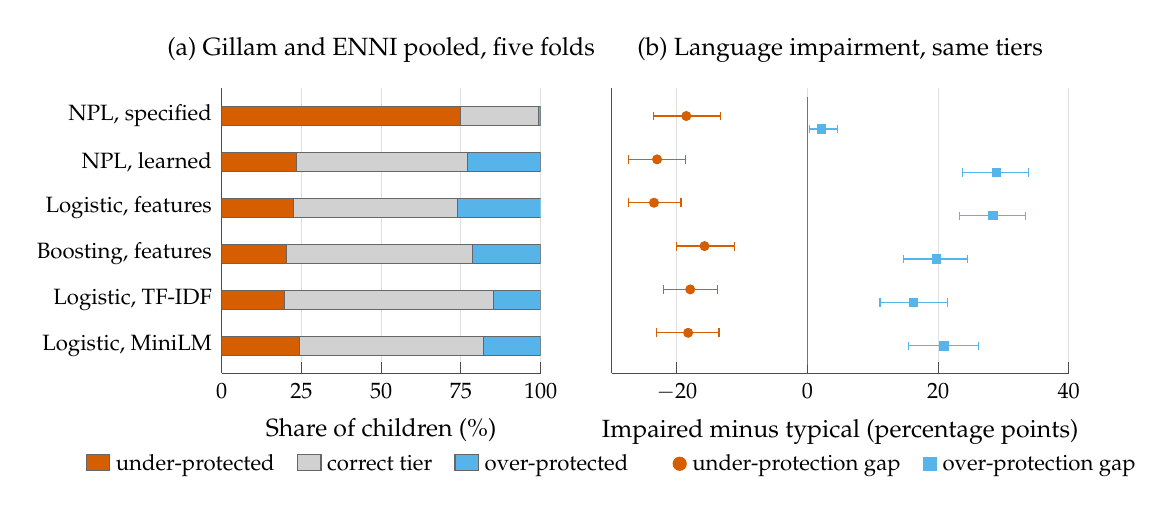
\begin{tikzpicture}
\begin{axis}[safenest, name=s1, 
  width=0.305\figwidth, height=52mm, scale only axis=false,
  xbar stacked, bar width=7pt, xmin=0, xmax=100, y dir=reverse,
  ytick={0,1,2,3,4,5}, yticklabels={{NPL, specified},{NPL, learned},{Logistic, features},{Boosting, features},{Logistic, TF-IDF},{Logistic, MiniLM}},
  enlarge y limits=0.12, xmajorgrids, xtick={0,25,50,75,100},
  xlabel={Share of children (\%)}, title={(a) Gillam and ENNI pooled, five folds},
]
\addplot[fill=accent, draw=black!60, line width=0.3pt] coordinates {(74.7,0) (23.4,1) (22.5,2) (20.3,3) (19.8,4) (24.5,5)};
\addplot[fill=black!18, draw=black!60, line width=0.3pt] coordinates {(24.5,0) (53.7,1) (51.4,2) (58.4,3) (65.4,4) (57.7,5)};
\addplot[fill=oksky, draw=black!60, line width=0.3pt] coordinates {(0.8,0) (22.9,1) (26.2,2) (21.3,3) (14.7,4) (17.8,5)};
\end{axis}
\begin{axis}[safenest, name=s2, at={($(s1.east)+(9mm,0)$)}, anchor=west,
  width=0.40\figwidth, height=52mm, y dir=reverse,
  xmin=-30, xmax=40,
  ytick={0,1,2,3,4,5}, yticklabels={}, enlarge y limits=0.12, ytick style={draw=none},
  xmajorgrids, xlabel={Impaired minus typical (percentage points)},
  title={(b) Language impairment, same tiers},
]
\draw[black!55, line width=0.5pt] (axis cs:0,-0.6) -- (axis cs:0,5.6);
\addplot[only marks, mark=*, mark size=1.6pt, accent,
  error bars/.cd, x dir=both, x explicit, error bar style={line width=0.5pt}]
  coordinates {(-18.55,-0.15) -= (5.06,0) += (5.17,0) (-23.03,0.85) -= (4.35,0) += (4.30,0) (-23.50,1.85) -= (3.94,0) += (4.14,0) (-15.76,2.85) -= (4.34,0) += (4.58,0) (-17.95,3.85) -= (4.08,0) += (4.19,0) (-18.27,4.85) -= (4.81,0) += (4.72,0)};
\addplot[only marks, mark=square*, mark size=1.5pt, oksky,
  error bars/.cd, x dir=both, x explicit, error bar style={line width=0.5pt}]
  coordinates {(2.19,0.15) -= (1.90,0) += (2.34,0) (28.91,1.15) -= (5.11,0) += (4.92,0) (28.38,2.15) -= (5.15,0) += (5.01,0) (19.73,3.15) -= (4.99,0) += (4.74,0) (16.24,4.15) -= (5.14,0) += (5.18,0) (20.88,5.15) -= (5.38,0) += (5.31,0)};
\end{axis}
\node[anchor=north, font=\footnotesize] at ($(s1.south)!0.5!(s2.south)+(0,-9mm)$) {%
  \tikz\fill[accent, draw=black!60] (0,0) rectangle (3mm,2mm);~under-protected\quad
  \tikz\fill[black!18, draw=black!60] (0,0) rectangle (3mm,2mm);~correct tier\quad
  \tikz\fill[oksky, draw=black!60] (0,0) rectangle (3mm,2mm);~over-protected\qquad
  \tikz\fill[accent] (0,0) circle (0.9mm);~under-protection gap\quad
  \tikz\fill[oksky] (0,0) rectangle (1.8mm,1.8mm);~over-protection gap};
\end{tikzpicture}
\end{document}
